%\chapter{Proof of Concept Design and Implementation}
%\chapter{Pixel-based Synthesis of 360\degree Viewpoints}
%\chapter{Pixel-based Synthesis of 360\degree Viewpoints with 2DoF}
\chapter{Pixel-based Rendering of 360\degree Viewpoints with 2DoF}
\section{Approach}
%\begin{itemize}
%  \item most other approaches rely on either geometry or correspondences
%  \item usually some form of triangulation
%  \item use of sphere for ray tracing, then use texture lookup to find the pixel values
%  \item combination of reprojection ie warping with angle constraint and flow-based blending
%  \item first part relies on radius/scale, but no geometry, second part relies on image correspondences
%  \item ``view-dependent texture maps'' \ar environment map / viewpoint is chosen based on some kind of proximity to the synthesized view
%  \item pixel-based, in that each pixel is calculated separately, there are not image-area based constraints
%\end{itemize}

\subsection{Assumptions}
\begin{itemize}
  \item all images are oriented the same
  \item all images were captured on a plane parallel to the floor
  \item the positions of the captures are known
  \item the scale (radius) of the scene is known
  \item all synthesized viewpoints are located inside the scene boundaries
\end{itemize}

\subsection{Basic 2DoF Synthesis}
With these assumptions and using a basic model geometry with the same scale as the captured scene, it is already possible to synthesize new views of varying accuracy, depending on the scene. The process presented here for basic 2 degree of freedom synthesis is a combination of texture lookup through raytracing, and mosaicking by using a deviation angle constraint.

\subsubsection{Raytracing-based Texture Lookup}
The first step is to map the texture (i.e. pixel values) of an existing viewpoint to a new viewpoint according to its position in the scene. Theoretically, any 360\degree viewpoint can be mapped to any other, since each 360\degree image captures each point in the scene. This is only theoretically the case, since image resolution and occlusions in the scene will conceal some areas for some viewpoints whereas they are visible for others. However, at this point, this will be ignored and it will be assumed that each viewpoint image contains all the points of the scene albeit at different image coordinates and different sampling rates\footnote{By design, areas closer to the camera are captured with a higher sampling rate per point than areas farther away.}. 

Additionally, 3D geometry of the scene is needed for raytracing. However, since the approach in this thesis does not capture or infer any real geometry, a model geometry is used that has approximately the same scale as the scene that was captured. The model geometry is a sphere, as this is a simple, very general geometry to represent a variety of different scenes. The radius of the sphere is chosen so that the sphere contains all possible points in the scene, for which the scale of the scene needs to be known. Under these assumptions, it is possible to map the image at one viewpoint to a new position by combining raytracing and texture lookup.

% This is visualized in Figure~\ref{fig:reflected_rays} a: Each point P of the scene reflects light rays in all directions. These light rays are captured at different viewpoints and are discretized into pixels in the image taken at that viewpoint. As a result, the pixels representing point P are present in the images captured at each viewpoint. This means that when synthesizing a new viewpoint S, the pixels representing point P can theoretically be retrieved from any of the images at the captured viewpoints (Figure~\ref{fig:reflected_rays} b).
%\begin{figure}[]
%\centering
%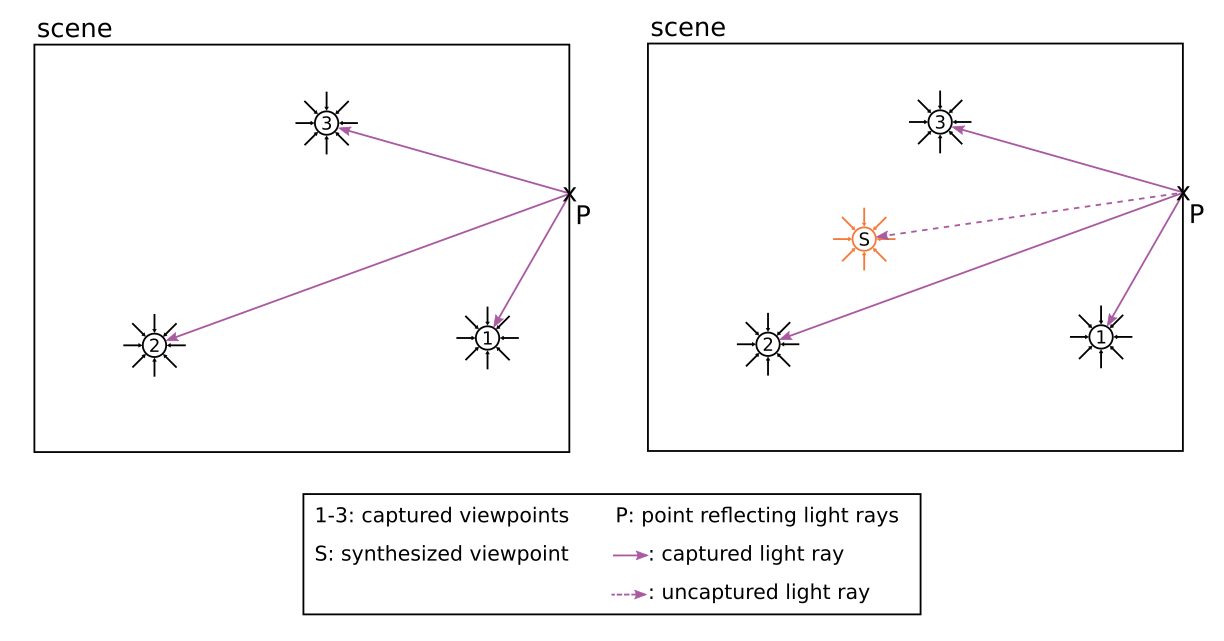
\includegraphics[width=1\textwidth]{03/incoming_lightrays.png}
%\caption[Light rays reflected from a point in the scene]{The reflected light rays from each point in the scene are captured by each 360\degree viewpoint}
%\label{fig:reflected_rays}
%\end{figure}

In order to do this, several steps of raytracing are necessary, which are visualized in Figure~\ref{fig:raytracing}. Figure~\ref{fig:raytracing}a shows how a camera at a specific viewpoint captures the light rays reflected from the objects in the scene. The captured pixel values are visualized on a circle around the center of projection of the camera (for simplicity's sake, only one row of pixels is shown). Once the viewoints have been captured (there is only one viewpoint in this example), a new viewpoint is ready to be synthesized. The model geometry is visualized as a circle\footnote{In this example, the model sphere does not surround the complete scene (the corners of the scene are outside of the circle). This is only for visualization purposes, normally the sphere would contain the complete scene, including the corners.} in Figure~\ref{fig:raytracing}b, with the new viewpoint to be synthesized represented by a dotted circle around a center of projection. For each pixel of the synthesized image, a ray is projected into the scene (Figure~\ref{fig:raytracing}c) and its intersection with the scene is calculated. Then, the ray from the center of projection of the captured viewpoint to the scene intersection is calculated and the pixel value at that position in world coordinates is retrieved (Figure~\ref{fig:raytracing}e) and copied back to the new viewpoint (Figure~\ref{fig:raytracing}f). This way, the pixel values (i.e. texture) of a captured viewpoint are mapped to the new viewpoint (Figure~\ref{fig:raytracing}g). Figure~\ref{fig:raytracing}h compares the mapped values to the actual scene. It is immediately visible that most points have the value they would have, had the viewpoint been captured instead of synthesized (ground truth value), whereas some are incorrect. This is due to the disparity between the model and the real scene.

\begin{figure}
\centering
    \hfill
    \begin{subfigure}[t]{0.3\textwidth}            
            \centering
            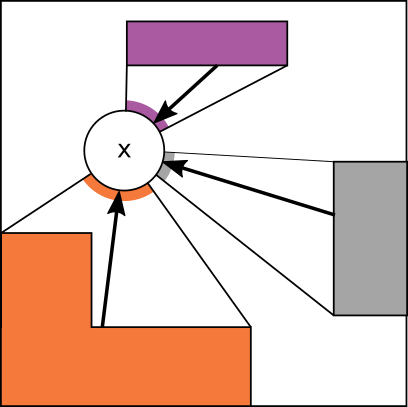
\includegraphics[width=0.9\textwidth]{03/raytracing01.png}
            \caption{The real scene viewed from above: The camera captures light rays reflecting from objects}
    \end{subfigure}%
    \hfill
     %add desired spacing between images, e. g. ~, \quad, \qquad etc.
      %(or a blank line to force the subfigure onto a new line)
    \begin{subfigure}[t]{0.3\textwidth}
            \centering
            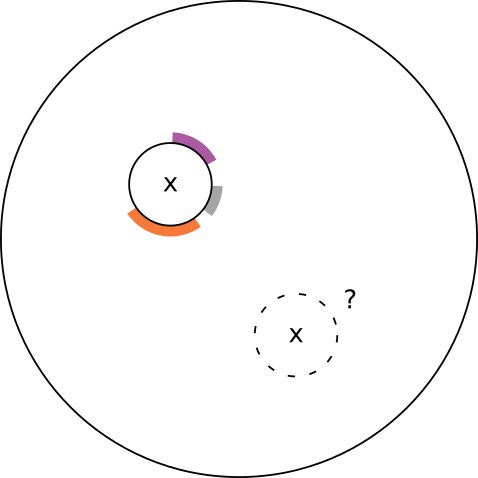
\includegraphics[width=0.9\textwidth]{03/raytracing02.png}
            \caption{A new viewpoint to be synthesized using the model geometry (sphere)}
    \end{subfigure}
    \hfill
    \hfill

    \hfill
    \begin{subfigure}[t]{0.3\textwidth}            
            \centering
            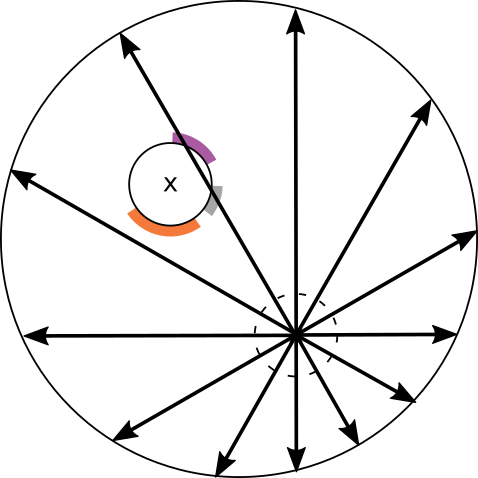
\includegraphics[width=0.9\textwidth]{03/raytracing03.png}
            \caption{A ray for each pixel in the synthesized viewpoint is traced to its intersection with the model}
    \end{subfigure}%
    \hfill
    \begin{subfigure}[t]{0.3\textwidth}
            \centering
            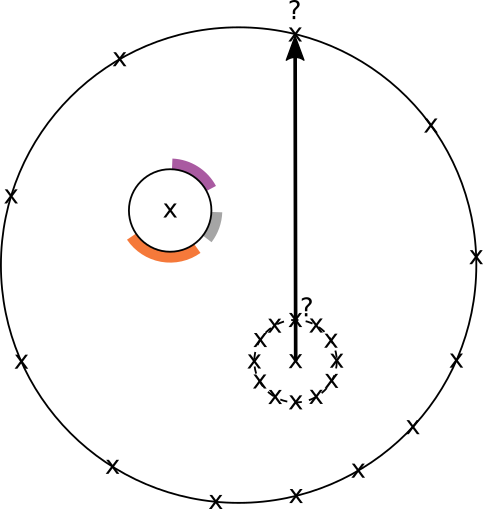
\includegraphics[width=0.9\textwidth]{03/raytracing04.png}
            \caption{For each ray, a texture lookup is performed}
    \end{subfigure}
    \hfill
    \begin{subfigure}[t]{0.3\textwidth}
            \centering
            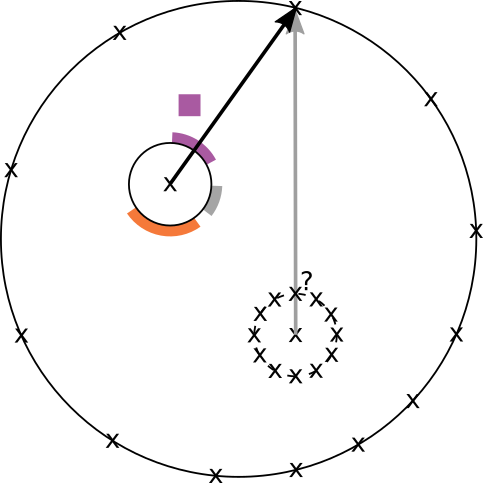
\includegraphics[width=0.9\textwidth]{03/raytracing05.png}
            \caption{From the ray-model intersection, a second ray is traced to the center of projection of the captured viewpoint and the pixel value is looked up}
    \end{subfigure}
    \hfill

    \hfill
    \begin{subfigure}[t]{0.3\textwidth}            
            \centering
            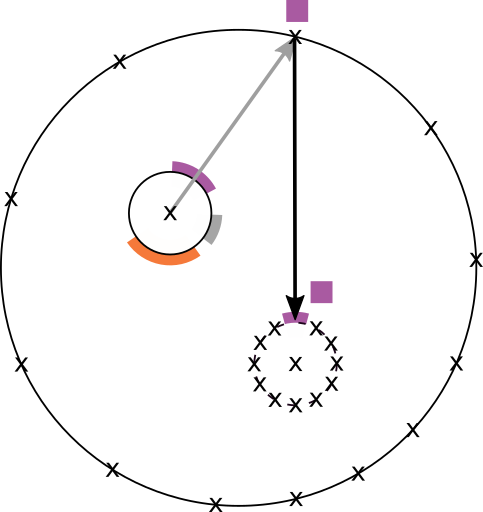
\includegraphics[width=0.9\textwidth]{03/raytracing06.png}
            \caption{The pixel value is copied back to the new viewpoint}
    \end{subfigure}%
    \hfill
    \begin{subfigure}[t]{0.3\textwidth}
            \centering
            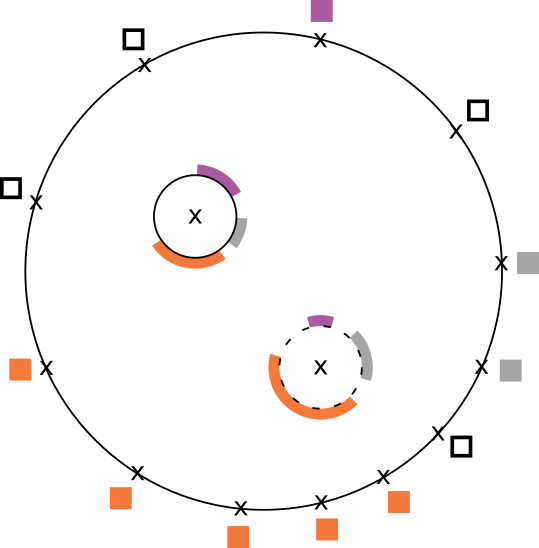
\includegraphics[width=0.9\textwidth]{03/raytracing07.png}
            \caption{This process is repeated for all pixels}
    \end{subfigure}
    \hfill
    \begin{subfigure}[t]{0.3\textwidth}
            \centering
            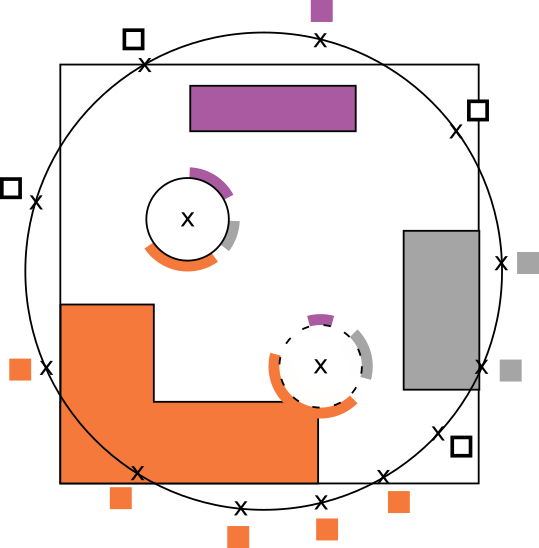
\includegraphics[width=0.9\textwidth]{03/raytracing08.png}
            \caption{The resulting texture mapping from the captured viewpoint to the model geometry in comparison with the original scene}
    \end{subfigure}
    \hfill
    \caption[Texture lookup through raytracing]{Process of texture lookup through raytracing}\label{fig:raytracing}
\end{figure}

%The basic idea of the 2/3DoF algorithm is to find the image areas from the set of existing viewpoints that are the ``most fitting'' for the synthesized viewpoint and transform these areas to approximate where they would be in the synthesized image. This means that a metric is necessary that measures how ``fitting'' a specific pixel of a viewpoint image is. Also, a reprojection needs to be found that transforms the ``fitting'' image areas to the appropriate image coordinates for the synthesized viewpoint.
%\missingfigure{point correspondences and reprojection intro}


\subsubsection{Deviation-angle-based Mosaicking}
The example in Figure~\ref{fig:raytracing} contains only one captured viewpoint, so the choice of which viewpoint to use for texture lookup is trivial. In cases where several viewpoints are available, a choice must be made as to which viewpoint should be used. In the case where the real scene has the same geometry as the model sphere, this is practically irrelevant, since the raytracing is always accurate. However, this is unrealistic, since the number of spherical rooms containing no objects is negligible. As a result, as soon as the real scene differs from the model sphere, some viewpoints are more appropriate than others. Figure~\ref{fig:dev_angle}a shows how a discrepancy between the real scene and the model sphere can lead to inaccurate results.

When considering appropriateness, two metrics can be examined: the euclidean distance of a captured viewpoint from the synthesized viewpoint, and the deviation angle between the rays. Figure~\ref{fig:dev_angle}b compares the two metrics and in the example it is evident that the deviation angle is more appropriate. In fact, assuming that there is no obscuring element in the air such as fog, and disregarding diffusion over distance, the same light ray is captured by any viewpoint located on that ray. Sampling rates and resolution also have an effect on the accuracy of this assumption but these will also be foregone at the moment.

With these assumptions, it is evident using the deviation angle as the metric for appropriateness on a per-pixel basis produces more accurate results than using the euclidean distance. As a result, depending on the number and relative location of the captured viewpoints, using a per-pixel, deviation-angle-based constraint leads to a synthesized image made up of patches from different viewpoints (i.e. mosaic). 

%Inspired by different approaches to view-dependent texture mapping from \cite{cv_book} and \cite{megastereo}

- different sections of different viewpoints may be more appropriate in terms of accuracy
- use deviation angle as constraint (other possibilities are also possible, such as a combination of deviation angle and distance)
- calculate deviation angle and blend the best 2 based on a blending function (inverse sigmoid)
%    \item to determine which viewpoints to use for which output image areas, use weighting function $W(viewpoint)$ that is dependent on specific properties of the input viewpoint (e.g. euclidean distance of locations)

\begin{figure}
\centering
    \hfill
    \begin{subfigure}[t]{0.3\textwidth}            
            \centering
            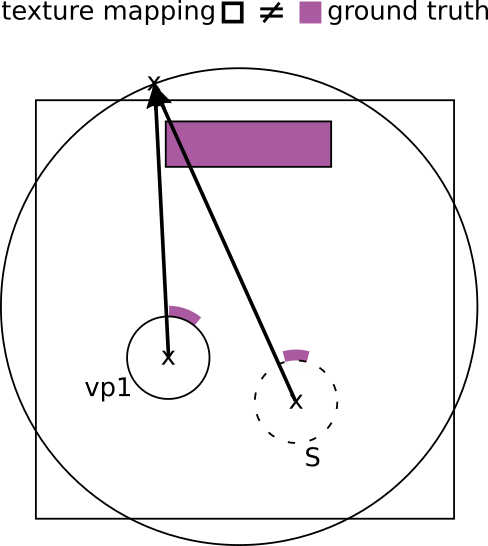
\includegraphics[width=0.9\textwidth]{03/dev_angles01.png}
            \caption{Differences in the real scene from the model can lead to incorrect remappings}
    \end{subfigure}%
    \hfill
     %add desired spacing between images, e. g. ~, \quad, \qquad etc.
      %(or a blank line to force the subfigure onto a new line)
    \begin{subfigure}[t]{0.3\textwidth}
            \centering
            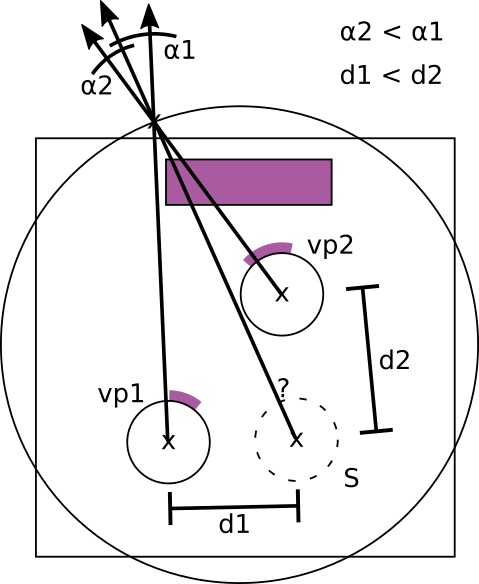
\includegraphics[width=0.9\textwidth]{03/dev_angles02.png}
            \caption{The deviation angle $\alpha$ of the rays can be compared, as well as the euclidean distance d}
    \end{subfigure}
    \hfill
    \hfill
    \caption[Choosing the appropriate viewpoint for texture lookup]{Choosing the appropriate viewpoint to improve the result} \label{fig:dev_angle}
\end{figure}
%In order to find the ``most fitting'' image area from all of the viewpoint images, there first needs to be a metric that measures how ``fitting'' an image area is. 

%One example is the euclidean distance of the viewpoint locations in space. This would mean that for each pixel, the corresponding pixel of the \emph{nearest viewpoint} would be used. This is the simplest approach, and would simply return the nearest neighbor. 

\subsection{2DoF Synthesis using Flow-based Blending}
Using basic 2DoF Synthesis works fairly well as long as the real scene geometry corresponds roughly to the model sphere. The basic shape of many rooms can be approximated by a sphere, however the objects within these rooms can diverge greatly from the model geometry. In these cases, ghosting and doubling artefacts become visible, such as areas appearing twice, not at all, or two areas overlapping inconsistently. This problem is exacerbated when the synthesized viewpoint is very close to an object, as is visualized in Figure~\ref{fig:flow-based-mot}: In this example the synthesized viewpoint is very close to a detailed object whose geometry diverges significantly from the model sphere. The values of the points captured by the two viewpoints $vp1$ and $vp2$ differ (orange and purple), and neither of them is the desired ground truth value (gray) (Figure~\ref{fig:flow-based-mot}a). In order to improve the result, an adapted variation of the flow-based blending method from Richardt et. al's Megastereo \cite{megastereo} is introduced. This method allows interpolation between two 360\degree viewpoints using optical flow. Figure~\ref{fig:flow-based-mot}b shows how the interpolation can be used to achieve a more accurate result: A new viewpoint $vp1-2$ is interpolated between $vp1$ and $vp2$ such that the interpolated viewpoint is located on the ray in question. This new viewpoint is then used for the texture lookup to create the synthesized image with the goal of improving the accuracy of the mapped point.

\begin{figure}
\centering
    \hfill
    \begin{subfigure}[t]{0.4\textwidth}            
            \centering
            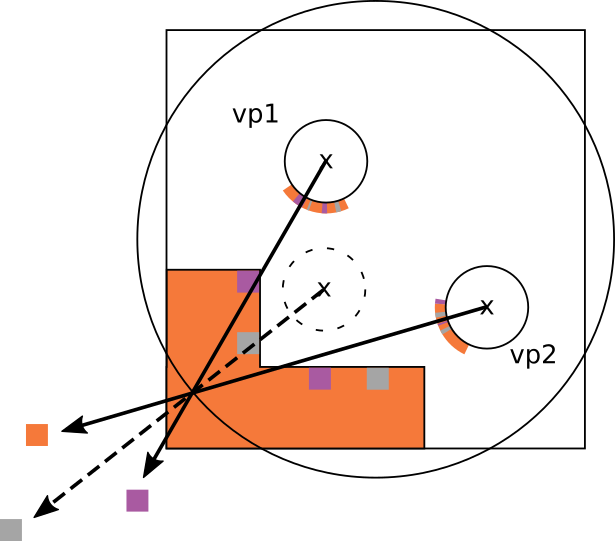
\includegraphics[width=0.9\textwidth]{03/flow-based01.png}
            \caption{Detailed areas where real geometry is very different from the model are problematic for basic 2DoF Synthesis}
    \end{subfigure}%
    \hfill
     %add desired spacing between images, e. g. ~, \quad, \qquad etc.
      %(or a blank line to force the subfigure onto a new line)
    \begin{subfigure}[t]{0.4\textwidth}
            \centering
            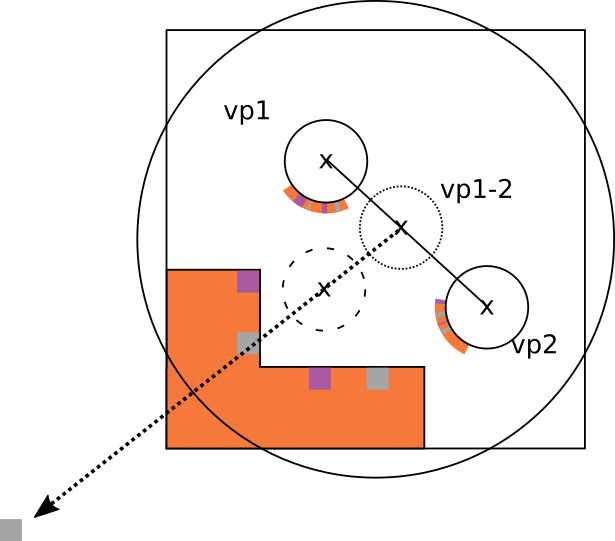
\includegraphics[width=0.9\textwidth]{03/flow-based02.png}
            \caption{Interpolating between input viewpoints using optical flow may improve results}
    \end{subfigure}
    \hfill
    \hfill
  \caption[Flow-based blending to improve accuracy in close, detailed areas]{Introducing flow-based blending to improve accuracy} \label{fig:flow-based-mot}
\end{figure}

%The simplest type of synthesis in the scope of this thesis is the creation of a new viewpoint that lies exactly on a line between two existing viewpoints. Assuming that the existing viewpoints are facing the same direction, the line describes a transformation with one degree of freedom, i.e. movement along the line. A solution to a similar problem has already been published by Richardt et al. in ``Megastereo'' \cite{megastereo} which introduces an approach using optical flow in order to reduce ghosting artefacts in planar images. The following section shows how the problem of 1D interpolation for 360\degree images can be reduced to the problem solved in Megastereo.

\subsubsection{Adapting Flow-based Blending in Megastereo for 360\degree Images}
Megastereo \cite{megastereo} aims to generate high-resolution stereo panoramas by combining images captured on a circle. Their approach is to combine corresponding strips of the captured images and to create a view for each eye (see Section \ref{megastereo}). In order to mitigate artefacts such as ghosting, they use ``flow-based blending'' to combine two images A and B. This consists of using the optical flow vectors $F_{A\rightarrow B}$ and their inverse $F_{B\rightarrow A}$. To get the interpolated image at position $\alpha$ between image A and B, first, image A is shifted by $\alpha \cdot F_{A\to B}$ and image B is shifted by $(1 - \alpha) \cdot F_{A\to B}$, yielding $I_A$ and $I_B$, respectively. Then, $I_A$ is multiplied by $(1-\alpha)$ and $I_B$ by $\alpha$ and these pixel values are added together to give the resulting interpolation. This is described by the following function, in which each pixel at position x of the synthesized image S is defined by: 

\begin{align}
S(x) &= (1-\alpha ) \cdot A( x + \alpha \cdot F_{A\to B}(x)) \nonumber\\
     &\qquad {} + \alpha \cdot B( x + (1-\alpha) \cdot F_{B\to A}(x))
\end{align}

%\subsubsection{Reducing 360\degree Interpolation to Planar Interpolation}
The flow-based blending in Megastereo operates on planar images. In order to use it for 360\degree synthesis, it is necessary to adapt the method for 360\degree images.

A 360\degree image can be projected in several ways, as described in Section \ref{projections}. The output of these projections is a planar image, meaning that it would be possible to apply flow-based blending directly. However, optical flow algorithms are generally designed to handle planar images without seams or distortions and would most likely produce unexpected results if used naively on planar projections of 360\degree images. As a result, the 360\degree images must first be projected and adapted in such a way that optical flow can be calculated accurately on them.

%Most projections distort the image in some areas, which would result in distorted optical flow values, e.g. the areas towards the poles in the equirectangular projection. Furthermore, in order to make planar viewing possible, the 360\degree image must be ``unfolded'' along some seam. When calculating optical flow, points that move across the seam will not be tracked, even though they do not move out of the image space, as would happen in a regular image.

Of the projections presented in Section~\ref{projections}, only the cubemap representation is applicable. Spherical representations are impractical, as aligning seams is not feasible and the distortion towards the edges is extreme. The equirectangular representation has only four seams to handle, but also distorts the image greatly around the poles. The cubemap representation contains a number of seams but does not distort the image more than a planar image would be. 
The challenge presented by the many seams of the cubemap is to be able to track points that move across the seams created by the six faces. Figure~\ref{fig:flow_seams} shows an example of different points moving across seams, illustrating why calculating optical flow on each face separately would not be enough. Figure~\ref{fig:flow_seams} also shows the linear discontinuities at the seams (e.g. at the upper edge of the carpet): since each cube face was captured by a different virtual camera, angles are not consistent across seams. As a result it is not possible to use the cube map as it is, since the optical flow assumes linear movement\footnote{Optical flow uses vectors to describe movement, which are inherently linear}.
%In order to handle points moving across seams, the optical flow algorithm must be able to read data \emph{across the seams}. 

%For example, when calculating optical flow on the ``front'' face, data from the ``top'', ``left'', ``right'' and ``bottom'' faces is required. Intuitively, one might just assemble these faces in a plus shape, with the ``front'' face at the center. However, this is a fallacy, since the cubemap projection uses a different virtual camera for each face, which means that linearity is not preserved for points moving across seams.

\begin{figure}
\centering
    \hfill
    \begin{subfigure}[t]{0.5\textwidth}            
            \centering
            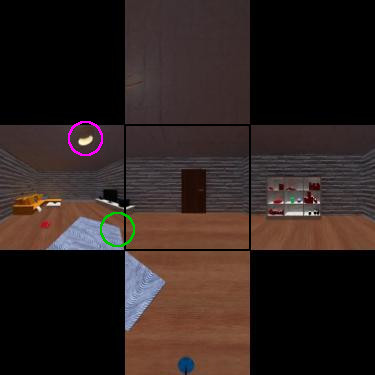
\includegraphics[width=0.9\textwidth]{03/flow_seams01.jpg}
            \caption{}
    \end{subfigure}%
    \hfill
     %add desired spacing between images, e. g. ~, \quad, \qquad etc.
      %(or a blank line to force the subfigure onto a new line)
    \begin{subfigure}[t]{0.5\textwidth}
            \centering
            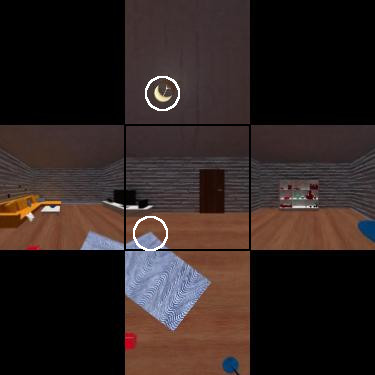
\includegraphics[width=0.9\textwidth]{03/flow_seams02.jpg}
            \caption{}
    \end{subfigure}
    \hfill
    \hfill
  \caption[]{Points in the scene moving across seam edges need to be tracked by optical flow (the back face of the cube map was omitted for simplicity's sake} \label{fig:flow_seams}
\end{figure}


To solve this problem, an ``extended cube map'' is used, which was also used by Huang et. al. \cite{6dof} to adapt 360\degree images for structure-from-motion algorithms. Instead of projecting a field of view of 90\degree for each camera, which covers 360\degree of the image, the extended cube map uses a larger field of view for each camera. As a result, the areas of the image that are split by a seam are represented twice: Once on each face that is adjacent to the seam. This way, when calculating optical flow on each face separately, points that move across where the seam would be in a regular cube map remain on the face with the corresponding projection. 

Naturally, this method is limited by the field of view used by the virtual cameras. If the maximum displacement is larger than the face extension, the extended cube map will not be sufficient, which will result in black edges on the faces. Also, the larger the field of view, the more the image will be distorted towards the edges of a face, which may lead to distorted optical flow results. This means that displacement between two images is limited. However, the displacement that is trackable by optical flow algorithms is also limited. The effect of these limitations will be explored in section \ref{evaluation1D}.

Using the extended cube map, it is possible to process each face separately, meaning that the 360\degree 1DoF interpolation has been reduced to planar images. At the end of the interpolation step, the extended cube map must be clipped back to the original cube map size.
\missingfigure{1D interpolation process diagram}

\subsubsection{Handling Multiple Input Viewpoints in Flow-based Blending}
- up until now: only 2 input viewpoints \ar 1DoF interpolation
- what to do with >2 viewpoints
- use min deviation angle again (+ distance?)

\section{Implementation}

\subsubsection{Preprocessing and CaptureSet}
\begin{itemize}
  \item rotate all images so that they all have the same orientation
  \item center point cloud
  \item find appropriate sphere radius
  \item make access to location and image data of a viewpoint contained in a set easy and intuitive
\end{itemize}

\subsubsection{Interpolation}
\begin{itemize}
  \item ray and scene intersection
  \item viewpoint reprojection
  \item deviation angle calculation
  \item weighting function
\end{itemize}
%further points to include
%- inverting flow is non-trivial

\paragraph{Calculating Ray-sphere Intersection}
The vectors representing these rays can be easily derived from the \emph{world coordinates} of the image (see~Section~\ref{fundamentals_360}).

The intersections of these rays with the model geometry can be calculated analytically: The sphere representing the scene can be represented implicitly by Equation~\ref{eq:rsi_spherefull}. The set of points P defined by this equation make up the surface of the sphere (Equation~\ref{eq:rsi_sphereP}). 
The equation describing any point on the ray can be expressed by Equation~\ref{eq:rsi_point}, where $O$ is the origin of the ray, which is the center of projection of the new viewpoint, $t$ is the length of the ray and $D$ is a unit vector describing the direction. 

\begin{align}
  x^2 + y^2 + z^2 - R^2 = 0&\label{eq:rsi_spherefull}\\ 
  P^2 - R^2 = 0&\label{eq:rsi_sphereP}
\end{align} 
\begin{align}
  P = O + tD& \label{eq:rsi_point}
\end{align} 

The point $P$ in Equation~\ref{eq:rsi_sphereP} can be substituted with the equation of the any point on the ray which yields Equation~\ref{eq:rsi_sub}. This equation can be developed into Equation~\ref{eq:rsi_quad}, which is a quadratic function with $a = D^2$, $b = 2OD$, $c = O^2-R^2$ (Equation~\ref{eq:quadf}).

\begin{align}
  |O + tD|^2 - R^2 &= 0  \label{eq:rsi_sub}\\
  D^2 t^2 + 2ODt + O^2 - R^2 &= 0 \label{eq:rsi_quad}
\end{align}

\begin{align}
  a = D^2, b = 2OD, c = O^2-R^2 \\
  f(t) = at^2 + bt + c \label{eq:quadf}\\
  t = \frac{-b \pm \sqrt{b^2 - 4ac}}{2a} \label{eq:solvequadf}
\end{align}

This equation can then be solved for t. Since the radius of the sphere is chosen so that it contains the complete scene and no viewpoints are synthesized outside of the scene, the quadratic function will always have two solutions (i.e. two intersections): one for which the vector length $t$ is negative, and one for which the vector length is positive. The positive value is used to find the intersection in question.

\subsection{Debugging and Verification}
\begin{itemize}
  \item in order to verify correct results and check for bugs, use of the ``checkersphere'' in which the scene model exactly matches the scene \ar reprojection will yield exact results (excluding resolution)
  \item explain why it will yield correct results and why the resolution is not perfect
\end{itemize}

\subsection{Implementation challenges}
``one on each side''
\begin{itemize}
  \item define ``on either side'' for angles: split the circle in two 180\degree halves; one is positive, the other is negative
  \item selection of a viewpoint ``on either side'' \ar what if the viewpoint on one side has a very large deviation angle or does not exist?
  \item can it not exist if we are looking at the convex hull? Yes, if the point is exctly on the border
  \item possible solution: if none is found, use only one side
  \item what to do with zero degree difference? \ar only use zero, not the other (should be solved by the function that defines the 1D interpolation position)
\end{itemize}
using only 2D data
\begin{itemize}
  \item ``left and right'' only possible in 2D (can use signed angles)
  \item in 3D, finding viewpoint on ``either side'' becomes a lot more complex
  \item reducing viewpoints to 2D is simple, but scene model is still in 3D. simplifying scene model to 2D as well
\end{itemize}

errors that are unrelated to the algorithm:
\begin{itemize}
  \item slight displacement due to ExtendedCubeMap
  \item black edges due to latlong-cube conversion
  \item these need to be taken into account (normalized out)
  \item only an issue for flow-based because flow-based uses conversion, whereas regular does not
\end{itemize}

\subsection{Performance}
